\begin{figure}[H]
    \centering
    \begin{subfigure}{0.48\textwidth} 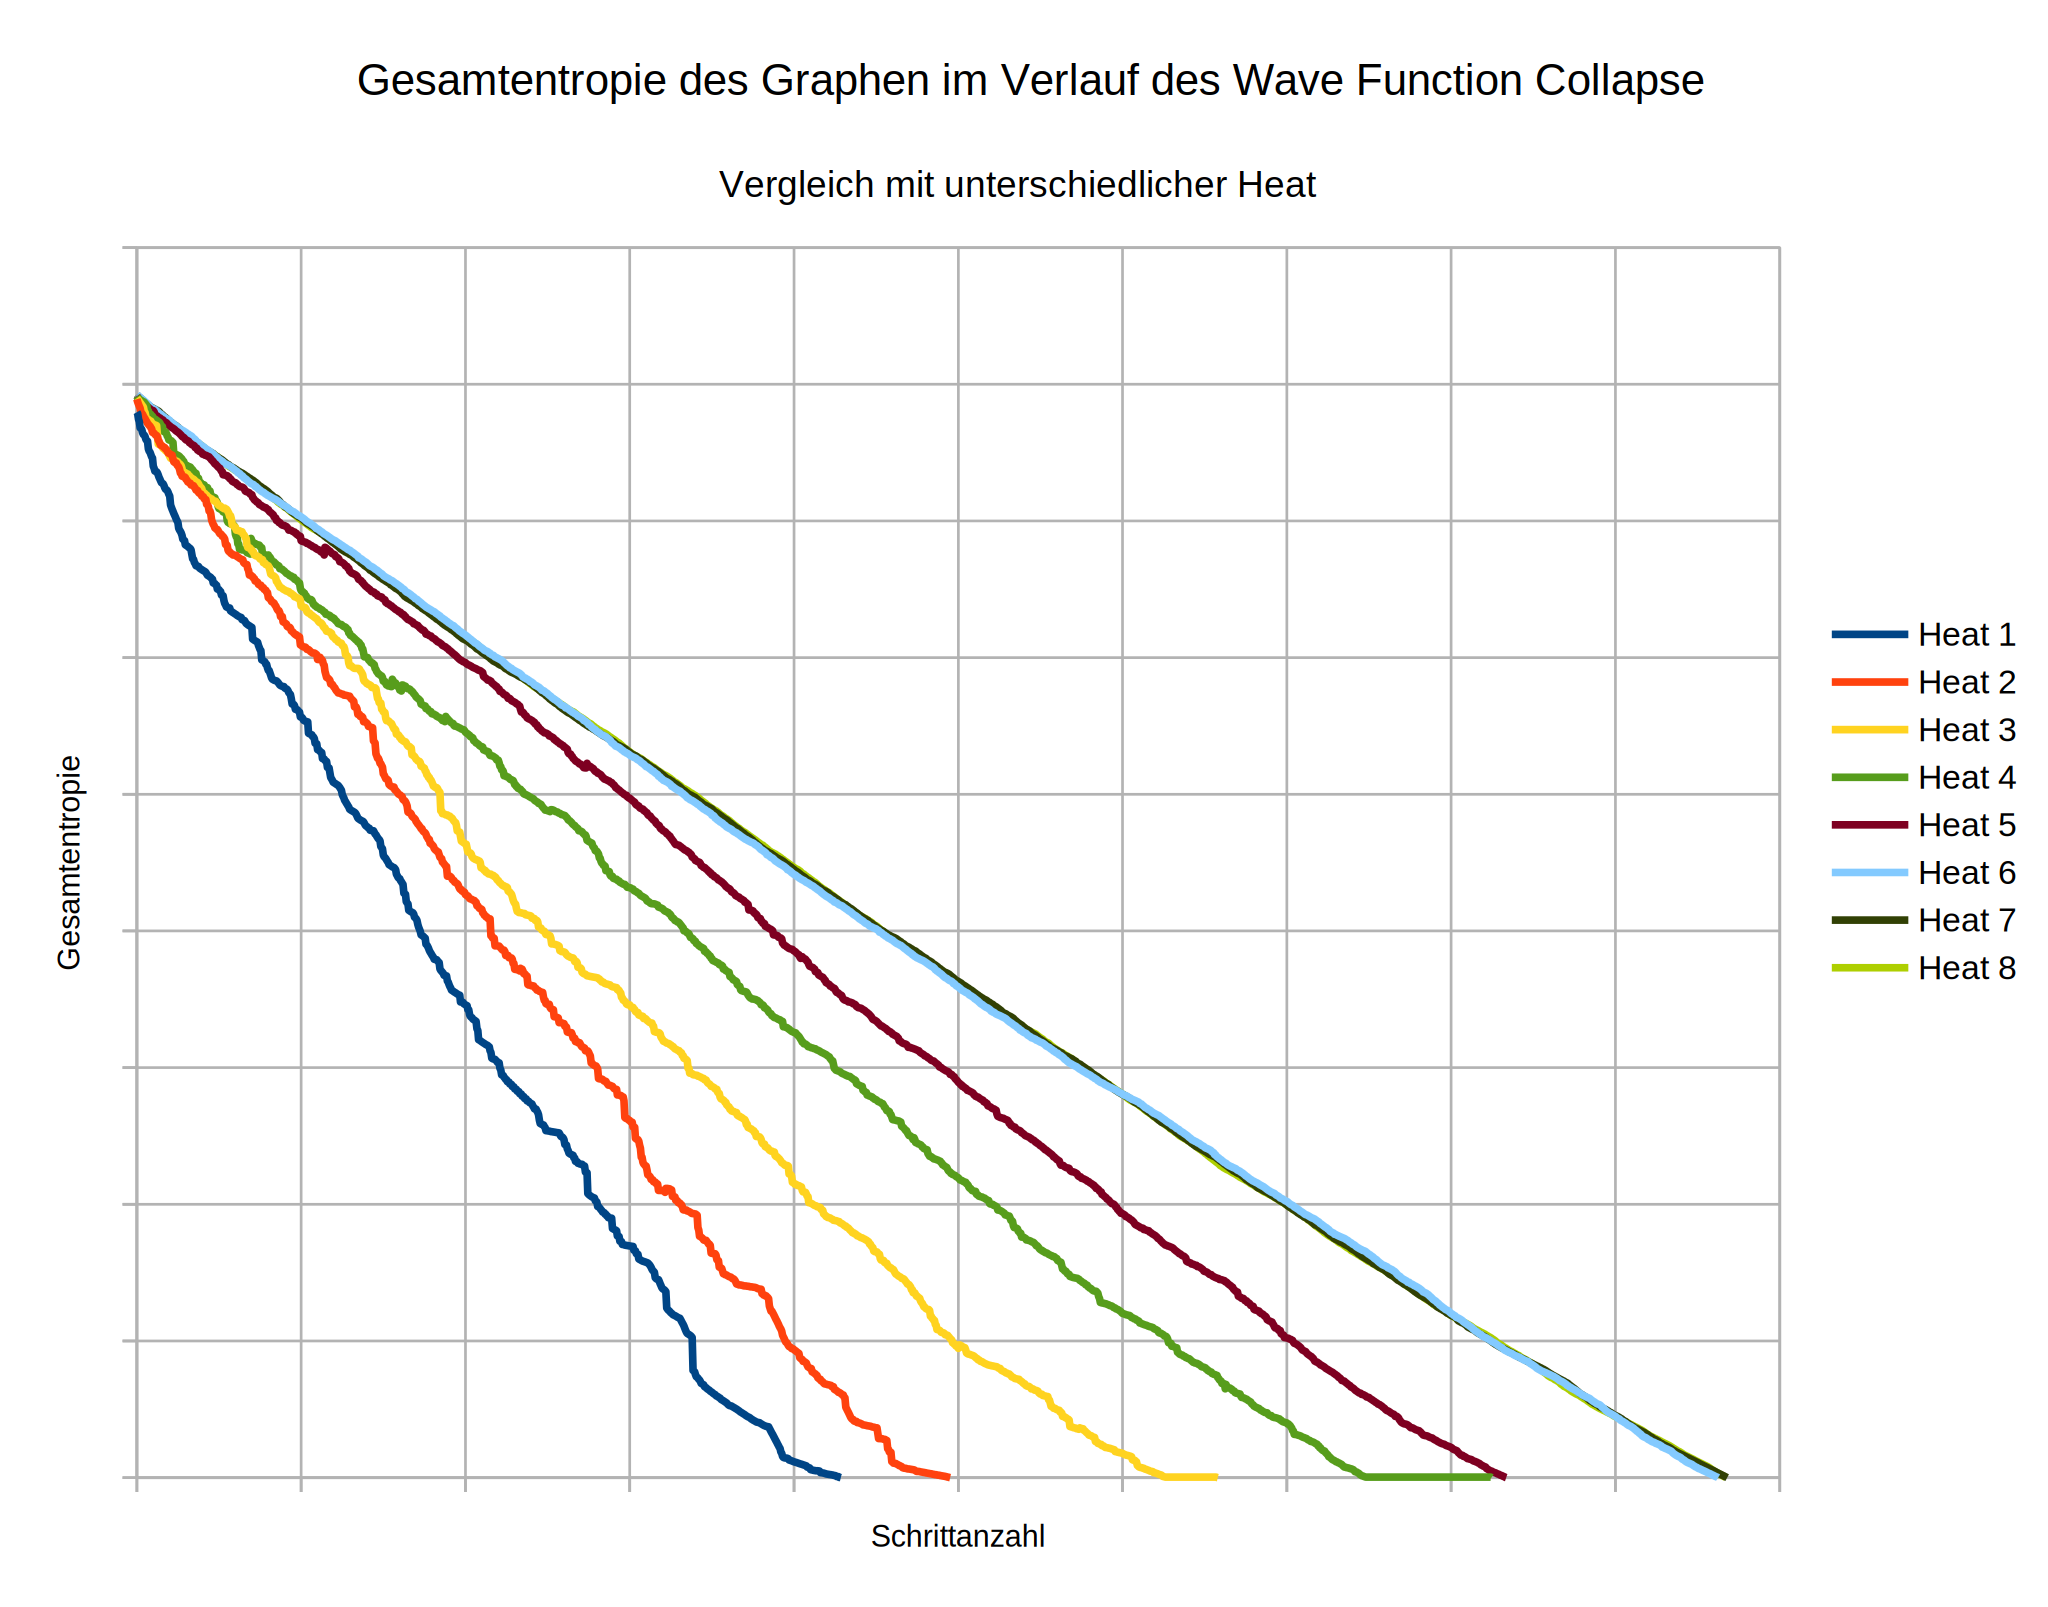
\includegraphics[width=\linewidth]{data/cell_size/1.png}  \caption{} \end{subfigure}
    \begin{subfigure}{0.48\textwidth} \includegraphics[width=\linewidth]{data/cell_size/2.png}  \caption{} \end{subfigure}
    
    \caption{
        Die Darstellung der Zellen im Graphen ist nicht nur auf die Voronoi-Zellen, wie in (a), beschränkt. In (b) werden die Zellen kleiner dargestellt.
    }
    \label{fig:cell_size}
\end{figure}